For the analysis of results gathered in our \textit{Evaluation Study}, we used R \cite{REnvironment} which is a well-known language and environment for statistical computing. We conducted non-parametric Kruskal-Wallis tests \cite{kruskal1952use} in order to verify the statistical relevance of our results. A Kruskal-Wallis test gives information about the likelihood that samples originate from the same distribution or not. In our case, we are evaluating this test on each individual testing variable (error rate, completion time, confidence) for all user groups (visualization types). The output of a Kruskal-Wallis test is a p-value which represents the probability that the labeled samples are from the same distribution. Hence, the smaller this p-value is, the higher is the probability that there are some differences between the individual groups. Our expectations for the results are formulated in the following hypotheses.

\begin{description}
\item[H1] Gradient Plots and Ambiguation Plots will perform better than just visualizing the mean value for the \textit{Probability Estimation} and \textit{Probability Comparison} tasks.
\item[H2] The visualization of means alone will result into a better and faster performance compared to Gradient Plots and Ambiguation Plots for the \textit{Average Comparison} tasks.
\item[H3] The \textit{Overlap Estimation} represents a mathematically more complex problem for which the quantitative result values can not be read directly from the visualizations we used in our study. Therefore we expect all three user groups to have problems with solving these tasks.
\end{description}

The following tables show the determined p-values of the Kruskal-Wallis tests for each testing variable and session. Table \ref{table:kruskal_all} contains the p-values for the whole result data, i.e. for all three user groups. Table \ref{table:kruskal_Gradient_Ambiguation}, \ref{table:kruskal_Gradient_Mean} and \ref{table:kruskal_Ambiguation_Mean} show the p-values for a pairwise comparison between Gradient and Ambiguation Plots, Gradient Plots and mean values, and Ambiguation Plots and means values respectively. This pairwise comparison was determined by conducting post-hoc Nemenyi-tests.


\begin{table}[H]
\centering
\resizebox{0.82\textwidth}{!}{
\begin{tabular}{|l|r|r|r|}
\hline
Task-type / p-value  & \textbf{Error-rate} & \textbf{Completion-time} & \textbf{Confidence} \\ \hline
\textbf{Probability Estimation} & 0.4425 & 0.5034 & 0.5973 \\ \hline
\textbf{Probability Comparison} & \cellcolor[HTML]{FFCB2F}{\color[HTML]{986536} \textbf{0.1954}} & 0.5199 & 0.7977 \\ \hline
\textbf{Average Comparison} & \cellcolor[HTML]{CE6301}{\color[HTML]{643403} \textbf{0.2414}} & \cellcolor[HTML]{009901}{\color[HTML]{013300} \textbf{0.09689}} & \cellcolor[HTML]{FFCB2F}{\color[HTML]{986536} \textbf{0.1686}} \\ \hline
\textbf{Overlap Estimation} & 0.8466 & 0.823 & 0.6358 \\ \hline
\end{tabular}}
\caption{\textit{The determined p-values on all testing variables and sessions, between all user groups.}}
\label{table:kruskal_all}
\end{table}

\begin{table}[H]
\centering
\resizebox{0.82\textwidth}{!}{
\begin{tabular}{|l|r|r|r|}
\hline
Task-type / p-value  & \textbf{Error-rate} & \textbf{Completion-time} & \textbf{Confidence} \\ \hline
\textbf{Probability Estimation} & 0.60 & 0.97 & 0.95 \\ \hline
\textbf{Probability Comparison} & 0.34 & 0.81 & 0.80 \\ \hline
\textbf{Average Comparison} & 0.71 & 0.89 & 0.99 \\ \hline
\textbf{Overlap Estimation} & 0.85 & 0.99 & 0.77 \\ \hline
\end{tabular}}
\caption{\textit{The determined p-values on all testing variables and sessions, between Gradient Plots and Ambiguation Plots.}}
\label{table:kruskal_Gradient_Ambiguation}
\end{table}

\begin{table}[H]
\centering
\resizebox{0.82\textwidth}{!}{
\begin{tabular}{|l|r|r|r|}
\hline
Task-type / p-value  & \textbf{Error-rate} & \textbf{Completion-time} & \textbf{Confidence} \\ \hline
\textbf{Probability Estimation} & 0.45 & 0.66 & 0.58 \\ \hline
\textbf{Probability Comparison} & 0.97 & 0.49 & 0.87 \\ \hline
\textbf{Average Comparison} & \cellcolor[HTML]{CE6301}{\color[HTML]{643403} \textbf{0.22}} & \cellcolor[HTML]{CE6301}{\color[HTML]{643403} \textbf{0.25}} & \cellcolor[HTML]{CE6301}{\color[HTML]{643403} \textbf{0.27}} \\ \hline
\textbf{Overlap Estimation} & 0.89 & 0.83 & 0.97 \\ \hline
\end{tabular}}
\caption{\textit{The determined p-values on all testing variables and sessions, between Gradient Plots and mean values.}}
\label{table:kruskal_Gradient_Mean}
\end{table}

\begin{table}[H]
\centering
\resizebox{0.82\textwidth}{!}{
\begin{tabular}{|l|r|r|r|}
\hline
Task-type / p-value  & \textbf{Error-rate} & \textbf{Completion-time} & \textbf{Confidence} \\ \hline
\textbf{Probability Estimation} & 0.97 & 0.50 & 0.77 \\ \hline
\textbf{Probability Comparison} & \cellcolor[HTML]{CE6301}{\color[HTML]{643403} \textbf{0.22}} & 0.85 & 0.99 \\ \hline
\textbf{Average Comparison} & 0.66 & \cellcolor[HTML]{009901}{\color[HTML]{013300} \textbf{0.099}} & \cellcolor[HTML]{CE6301}{\color[HTML]{643403} \textbf{0.21}} \\ \hline
\textbf{Overlap Estimation} & 1.00 & 0.88 & 0.63 \\ \hline
\end{tabular}}
\caption{\textit{The determined p-values on all testing variables and sessions, between Ambiguation Plots and mean values.}}
\label{table:kruskal_Ambiguation_Mean}
\end{table}

Additionally to this analytical evaluation with p-value tests, we also visually represent the gathered data with boxplots in order to give more information about the data's distribution properties. Figure \ref{fig:s1_boxplots}, \ref{fig:s2_boxplots}, \ref{fig:s3_boxplots} and \ref{fig:s4_boxplots} visualize the results for the \textit{Probability Estimation}, \textit{Probability Comparison}, \textit{Average Comparison} and \textit{Overlap Estimation} session respectively. For the creation of the boxplots, MATLAB \cite{MATLAB:2013} has been used.

\begin{figure}[H]
    \centering
    \begin{subfigure}[b]{0.32\textwidth}
        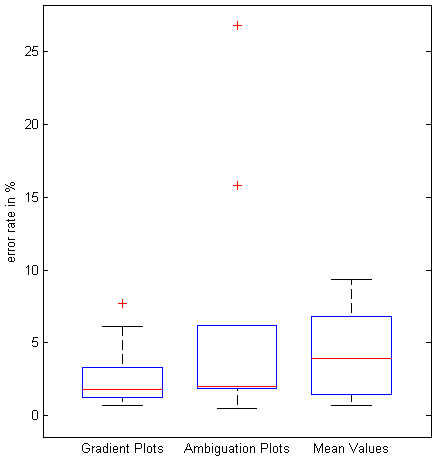
\includegraphics[width=\textwidth]{figures/boxplots/s1_error.png}
        \caption{Error rate}
        \label{fig:s1_error}
    \end{subfigure}
    \begin{subfigure}[b]{0.32\textwidth}
        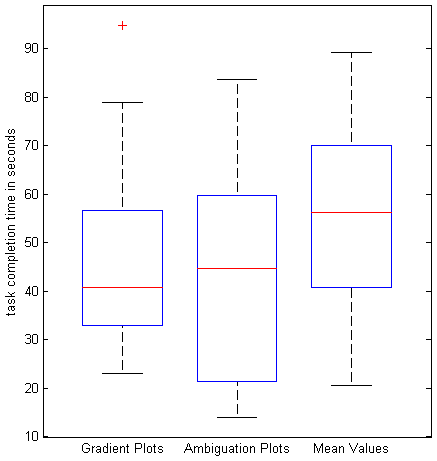
\includegraphics[width=\textwidth]{figures/boxplots/s1_time.png}
        \caption{Completion time}
        \label{fig:s1_time}
    \end{subfigure}
		\begin{subfigure}[b]{0.32\textwidth}
        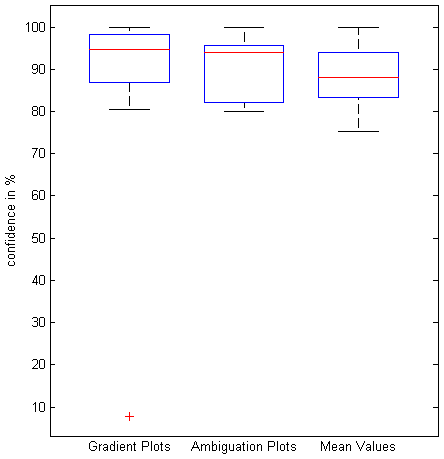
\includegraphics[width=\textwidth]{figures/boxplots/s1_confidence.png}
        \caption{Confidence}
        \label{fig:s1_confidence}
    \end{subfigure}
    \caption{Boxplots visualizing the gathered results of the Probability Estimation tasks.}
		\label{fig:s1_boxplots}
\end{figure}

\begin{figure}[H]
    \centering
    \begin{subfigure}[b]{0.32\textwidth}
        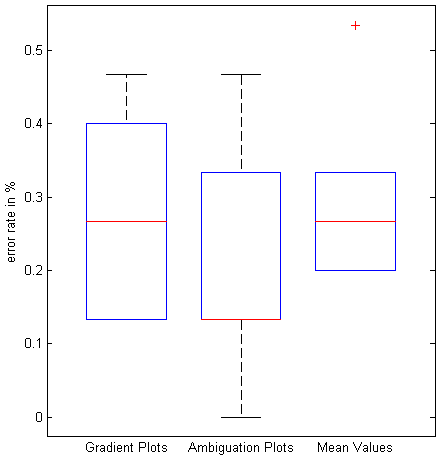
\includegraphics[width=\textwidth]{figures/boxplots/s2_error.png}
        \caption{Error rate}
        \label{fig:s2_error}
    \end{subfigure}
    \begin{subfigure}[b]{0.32\textwidth}
        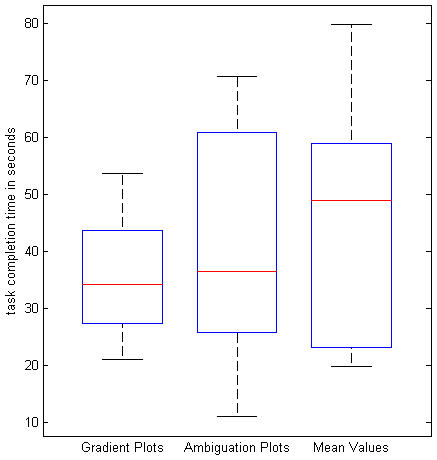
\includegraphics[width=\textwidth]{figures/boxplots/s2_time.png}
        \caption{Completion time}
        \label{fig:s2_time}
    \end{subfigure}
		\begin{subfigure}[b]{0.32\textwidth}
        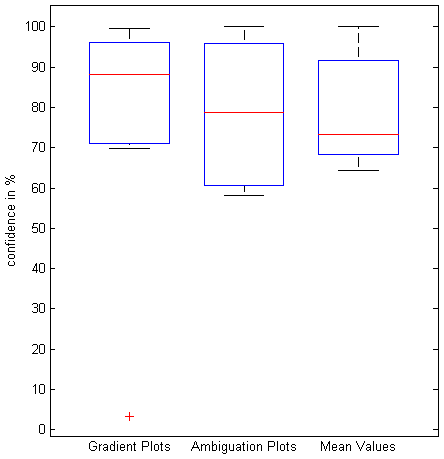
\includegraphics[width=\textwidth]{figures/boxplots/s2_confidence.png}
        \caption{Confidence}
        \label{fig:s2_confidence}
    \end{subfigure}
    \caption{Boxplots visualizing the gathered results of the Probability Comparison tasks.}
		\label{fig:s2_boxplots}
\end{figure}

\begin{figure}[H]
    \centering
    \begin{subfigure}[b]{0.32\textwidth}
        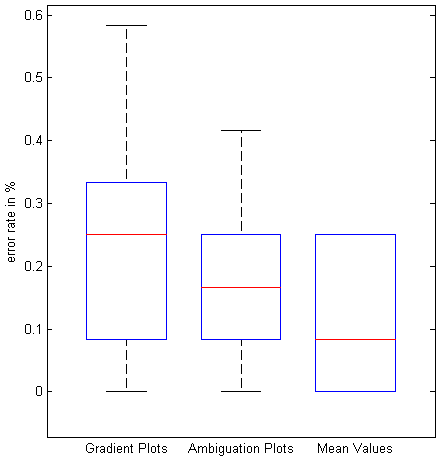
\includegraphics[width=\textwidth]{figures/boxplots/s3_error.png}
        \caption{Error rate}
        \label{fig:s3_error}
    \end{subfigure}
    \begin{subfigure}[b]{0.32\textwidth}
        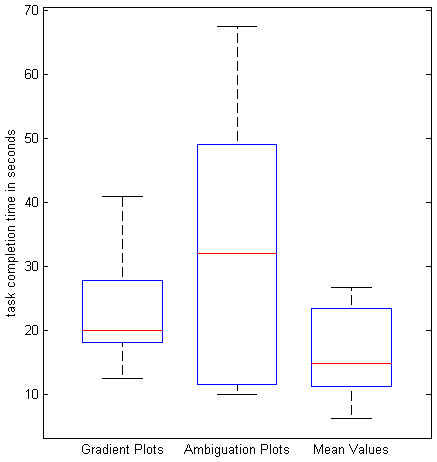
\includegraphics[width=\textwidth]{figures/boxplots/s3_time.png}
        \caption{Completion time}
        \label{fig:s3_time}
    \end{subfigure}
		\begin{subfigure}[b]{0.32\textwidth}
        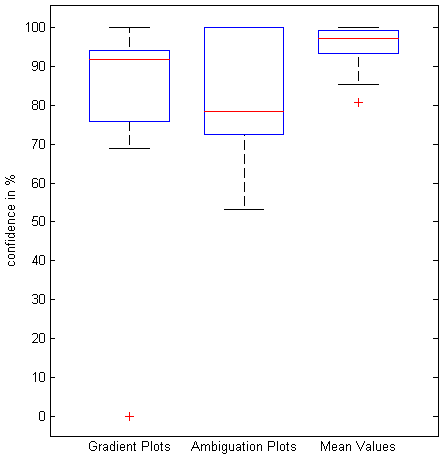
\includegraphics[width=\textwidth]{figures/boxplots/s3_confidence.png}
        \caption{Confidence}
        \label{fig:s3_confidence}
    \end{subfigure}
    \caption{Boxplots visualizing the gathered results of the Average Comparison tasks.}
		\label{fig:s3_boxplots}
\end{figure}

\begin{figure}[H]
    \centering
    \begin{subfigure}[b]{0.32\textwidth}
        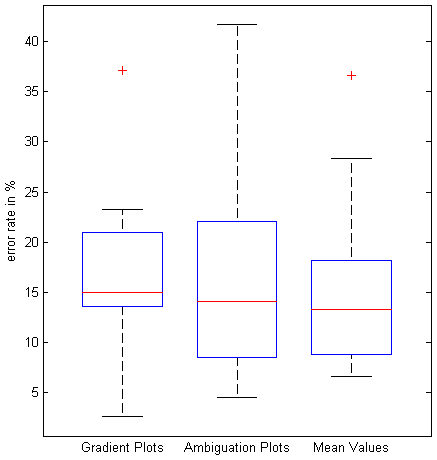
\includegraphics[width=\textwidth]{figures/boxplots/s4_error.png}
        \caption{Error rate}
        \label{fig:s4_error}
    \end{subfigure}
    \begin{subfigure}[b]{0.32\textwidth}
        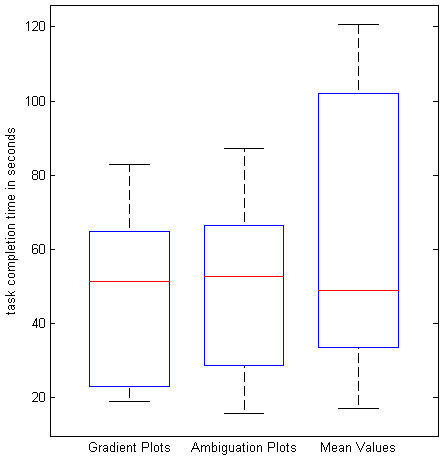
\includegraphics[width=\textwidth]{figures/boxplots/s4_time.png}
        \caption{Completion time}
        \label{fig:s4_time}
    \end{subfigure}
		\begin{subfigure}[b]{0.32\textwidth}
        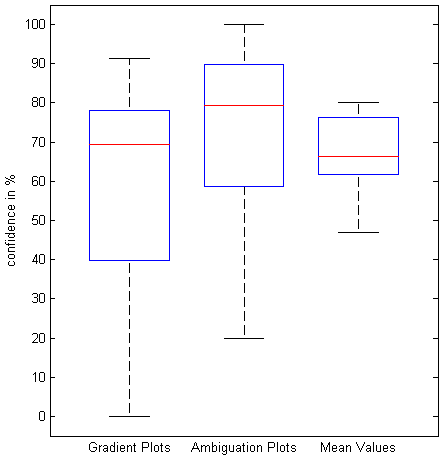
\includegraphics[width=\textwidth]{figures/boxplots/s4_confidence.png}
        \caption{Confidence}
        \label{fig:s4_confidence}
    \end{subfigure}
    \caption{Boxplots visualizing the gathered results of the Overlap Estimation tasks.}
		\label{fig:s4_boxplots}
\end{figure}